\documentclass[crop,tikz]{standalone}
\usepackage[subpreambles=true]{standalone}

\usepackage{pgf, tikz}
\usetikzlibrary{shapes.misc}
\usetikzlibrary{decorations.pathreplacing}

\tikzset{cross/.style={cross out, draw=black, minimum size=2*(#1-\pgflinewidth), inner sep=0pt, outer sep=0pt},
%default radius will be 1pt. 
cross/.default={0.25pt},
    point/.style={
    thick,
    draw=black,
    cross out,
    inner sep=0pt,
    minimum width=4pt,
    minimum height=4pt,
    },
}

\begin{document}

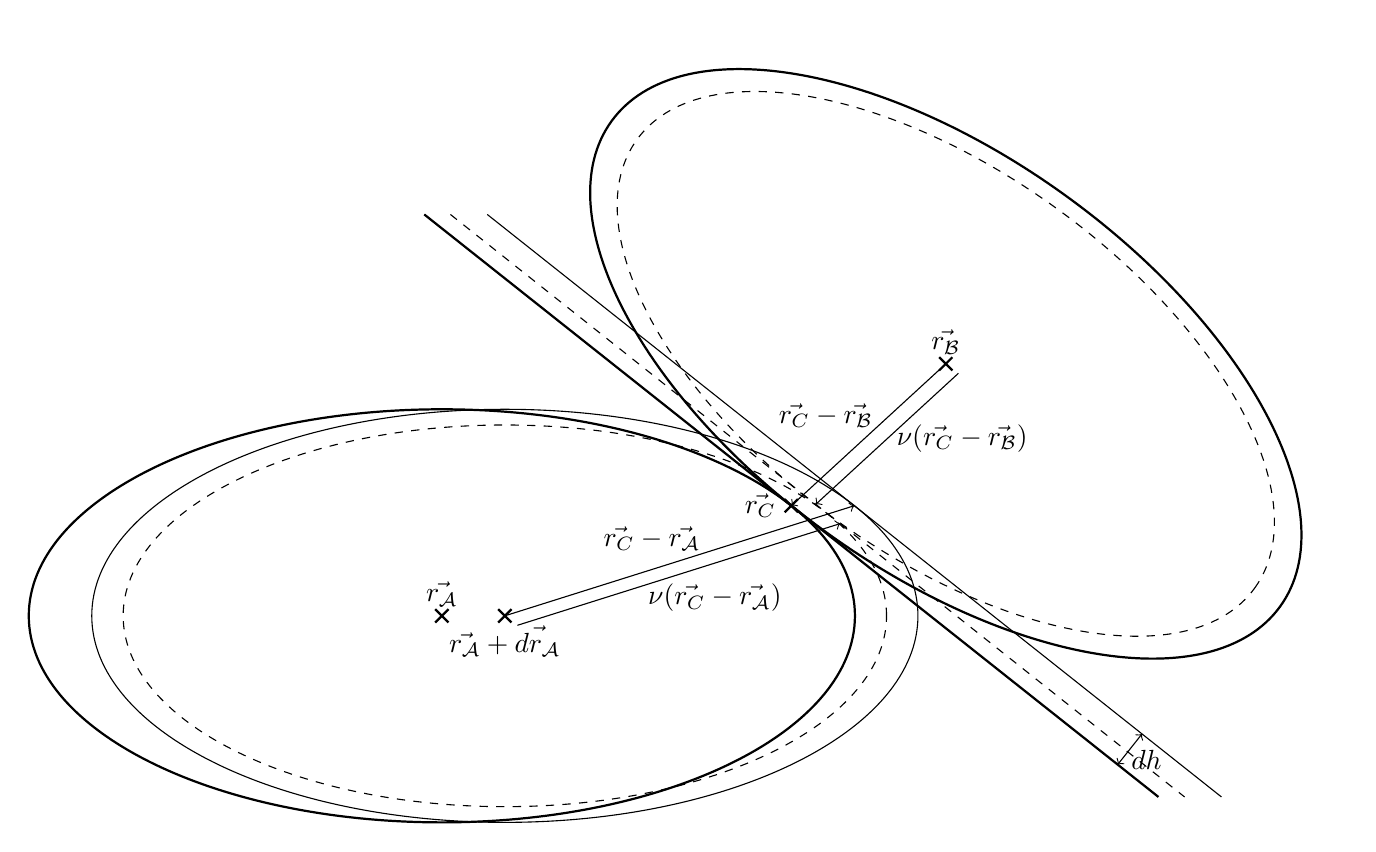
\begin{tikzpicture}[scale=8]
\node[point] at (0,0) {}; % rA
\draw (0,0) node[above]{$\vec{r_{\mathcal{A}}}$}; % rA
\node[point] at (0.1,0) {}; % rAdrA
\draw (0.1,0) node[below]{$\vec{r_{\mathcal{A}}} + \vec{dr_{\mathcal{A}}}$}; % rAdrA
\node[point] at (0.8,0.4) {}; % rB
\draw (0.8,0.4) node[above]{$\vec{r_{\mathcal{B}}}$};
\draw[thick] (0,0) ellipse (0.655762*1 and 0.655762*0.5); % ellipsoid A
\draw[thick, rotate around={-36:(0.8,0.4)}] (0.8,0.4) ellipse (0.655762*1 and 0.655762*0.5); % ellipsoid B
\draw[thick] (-0.02793517,  0.63719783) -- (1.13761317, -0.28753383); % contact plane
\draw (0.1,0) ellipse (0.655762*1 and 0.655762*0.5); % ellipsoid A displaced
\draw (-0.02793517 + 0.1,  0.63719783) -- (1.13761317 + 0.1, -0.28753383); % contact plane
%\draw[->] (0,0) -- (0.1,0) node[midway,below]{$\vec{dr_{\mathcal{A}}}$};
\draw[thin, dashed] (0.1,0) ellipse (0.605924*1 and 0.605924*0.5); % ellipsoid A
\draw[thin, dashed, rotate around={-36:(0.8,0.4)}] (0.8,0.4) ellipse (0.605924*1 and 0.605924*0.5); % ellipsoid B
\draw[dashed] (-0.02793517 + 0.0415,  0.63719783) -- (1.13761317 + 0.0415, -0.28753383); % contact plane
\draw[->] (0.1,0) -- (0.554839 + 0.1,0.174832) node[midway,above,xshift=-10pt]{$\vec{r_C} - \vec{r_{\mathcal{A}}}$};
\draw[->] (0.8,0.4) -- (0.554839,0.174832) node[midway,left,xshift=5pt,yshift=7pt]{$\vec{r_C} - \vec{r_{\mathcal{B}}}$};
\node[point] at (0.554839,0.174832) {};
\draw (0.554839,0.174832) node[left,xshift=-2pt]{$\vec{r_C}$};
%\draw[->] (0.11502684, -0.04768851) -- (0.554839*0.9238984255162129 + 0.11502684, 0.174832*0.9238984255162129 - 0.04768851) node[midway,below]{$\nu(\vec{r_C} - \vec{r_{\mathcal{A}}})$};
\draw[->] (0.1 + 0.01996544,0 - 0.01504598) -- (0.1 + 0.554839*0.9238984255162129 + 0.01996544,0.174832*0.9238984255162129 - 0.01504598)node[midway,below,xshift=13pt]{$\nu(\vec{r_C} - \vec{r_{\mathcal{A}}})$};
\draw[->] (0.8 + 0.01996544,0.4 - 0.01504598) -- (0.5934615781020197, 0.17692165932336534) node[midway,right]{$\nu(\vec{r_C} - \vec{r_{\mathcal{B}}})$};
%\draw[->] (0.8 - 0.01996544,0.4 + 0.01504598) -- (0.8 + 0.9238984255162129*(0.554839 - 0.8) + 0.01996544, 0.4 + 0.9238984255162129*(0.174832 - 0.4) - 0.01504598) node[midway,left]{$\nu(\vec{r_C} - \vec{r_{\mathcal{B}}})$};
% \draw[->] (0,0) -- (0.554839,0.174832) node[midway,below]{$\vec{r_C} - \vec{r_{\mathcal{A}}}$};
% \draw[->] (0.05,0.15) -- (0.554839 + 0.05,0.174832 + 0.15) node[midway,below]{$\vec{r_C} - \vec{r_{\mathcal{A}}}$};
% \draw[->] (0.8,0.4) -- (0.554839,0.174832) node[midway,right]{$\vec{r_C} - \vec{r_{\mathcal{B}}}$};
%\draw[<->] (1.07286048, -0.23615985) -- (1.07286048+0.09235021, -0.23615985+0.11639986) node[midway,above]{$dh$};
\draw[<->] (1.07286048, -0.23615985) -- (1.07286048+0.03863012, -0.23615985+0.0486901) node[midway,right,xshift = -3pt,yshift=-6.35 + 3*0.7933876513435727pt]{$dh$};
%0.03863012,  0.0486901
\end{tikzpicture}

\end{document}